\section{Working principle}%
\label{sec:working_principle}

\subsection{Microcontroller}%
\label{sub:microcontroller}
Programming of the MCU is historically conducted in the processor architecture's specific assembly language. Today, many MCUs support programming in several high-level languages where Embedded-C is one of the most common. Other alternatives, such as the Raspberry Pi Zero uses MicroPython which is an embedded-compatible dialect of Python. This allows for programming MCUs using the popular Python syntax wrapping around the C language. The Embedded-C language supports inline assembly code which is handy when the programmer wants section of code to be very specific and remain untouched by compiler optimizations.

% IMG
\begin{figure}[h]
  \centering
  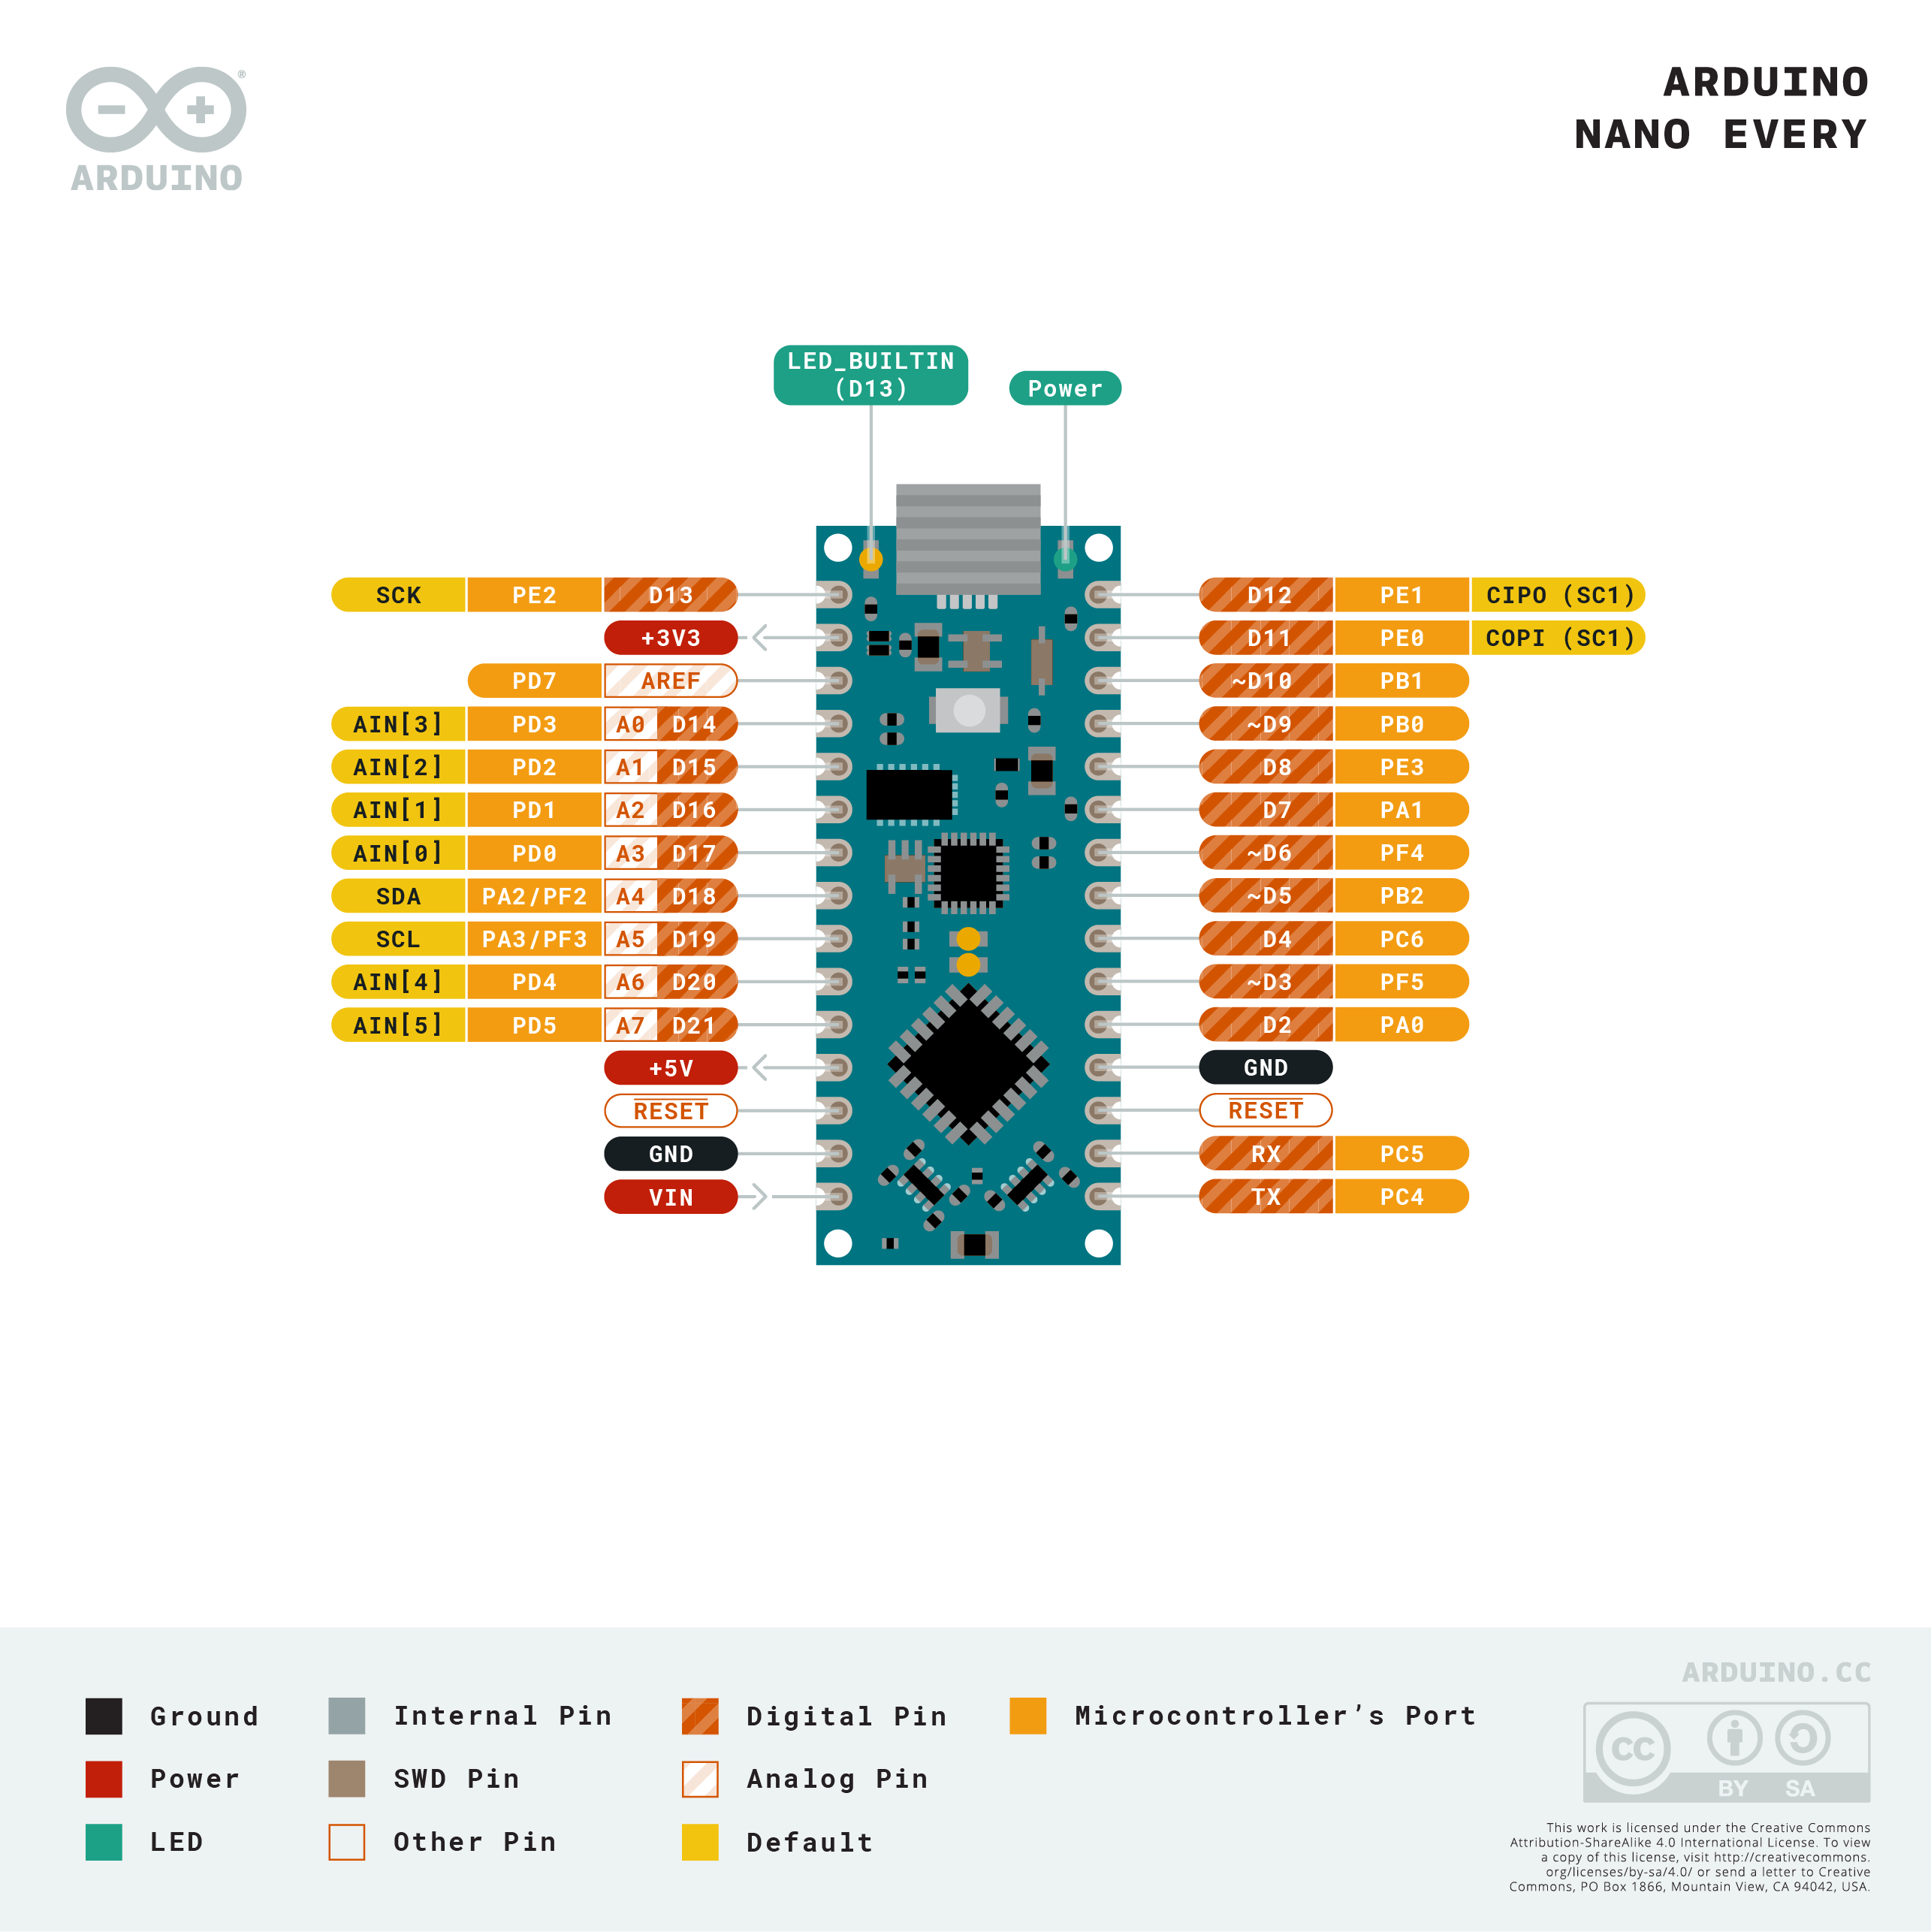
\includegraphics[width=0.8\textwidth]{/home/auan/Project/Report/Images/nano.png}
  \caption{Arduino Nano board layout \cite{PinoutNANO}}
  \label{fig:nano}
\end{figure}

According to the Figure \ref{fig:nano}, the ATmega328p (on the Arduino Nano) has different properties for analog or digital signals depending on the pin number. The Arduino is more or less a plug-and-play device if the proper drivers are installed for the USB interface connected to the programmer.

\subsection{Single-board computer}%
\label{sub:single_board_computer}
SBCs are a often cheap, lightweight and low-power alternative that contains many features of a PC on the system size of a debit card. One of the most notable manufacturers is Raspberry Pi whose latest models uses a multiprocessing 64-bit CPU, 1GB RAM and WLAN/Bluetooth networking capabilities. It is very useful for developing systems where a general purpose computers can fit inside a robot or scattering multiple units as a data collection network. There exists a multitude of lightweight open-source OS variants for the ARM architecture.

\subsection{Digital temperature sensor}%
\label{sub:digital_temperature_sensor}
A digital temperature sensor is an embedded system that is able to convert an analog reading of some physical property that varies proportionally when exposed to different temperatures. As the ADC conversion is done inside the sensor, the emphasis is not on the exact physical mechanisms of the but focuses on communicating using drivers written in Embedded-C.

\subsection{UART communication}%
\label{sub:uart}
An MCU can communicate with an SBC using the serial communication protocol UART \cite{trevennorPracticalAVRMicrocontrollers2012}. Depending on the application, or hardware specifications, it is possible to customize the UART signal window to contain several combination of start, stop and parity bits.
\begin{figure}[htpb]
  \centering

  \begin{tikztimingtable}
    [timing/d/background/.style={fill=white},
    timing/lslope=0.2,
    xscale=1.5,yscale=1.5]

    \texttt{UART} & H [dotted] ;HLL 8{2Q} HH;H [dotted]\\
    \extracode
    % Add vertical lines in two colors

    \begin{pgfonlayer}{background}
      \begin{scope}[semitransparent,semithick]
        \vertlines[dotted]{2.1,4.1,...,22.1}
        \foreach \i [count=\col from 0] in {2.1,4.1,...,22.1}
        \node[font=\scriptsize] at (\i,3) {$t_{\col}$};   
      \end{scope}
      \end{pgfonlayer}

  \end{tikztimingtable}
  \caption{The bitwise UART communication pattern}
  \label{fig:uartsig}
\end{figure}


As seen in \ref{fig:uartsig}, this example consists of a low start bit, eight data bits and a high stop bit.

\subsection{Web application}%
\label{sub:web_application}
A common way of constructing the front-end usually consists of 
\begin{enumerate}
  \item HTML -- constructing the web page document structure. A very simple text-based website can be constructed only using HTML. The page is then interpreted depending on the user's system defaults.
  \item CSS -- each element in the HTML document can either be styled individually or globally by defining a style-sheet. This handles elementary attributes such as colours, fonts, spacing and padding.  
  \item Scripting -- in order to perform work that handles computation of variables and automated tasks, it is often executed by some kind of script language. A common language for this purpose is JavaScript, or any of its super-sets such as TypeScript. This can also include calls to advanced APIs in order to for example get, process or present data in a certain way.

\end{enumerate}
By using scripts, that can handle real-time information from the user and web browser, it is possible to create highly dynamic web pages that graphically scales well to both stationary and mobile devices.
%When managing the back-end of a web application, it is important to choose a suitable database that is both compatible with the eventual APIs as well as the type of data it is containing. 

